\documentclass[12pt, a4paper]{book}

\usepackage{fancyhdr}
\usepackage[left=4cm, right=4cm, top=4cm, bottom=4cm]{geometry}
\usepackage[utf8]{inputenc}
\usepackage[table]{xcolor}
\usepackage{hyperref}
\usepackage{amsmath}
\usepackage{enumitem}
\usepackage[linewidth=1pt]{mdframed}
\usepackage{graphicx}
\usepackage{amsfonts}
\usepackage{centernot}
\usepackage{booktabs}
\usepackage{subcaption}
\usepackage[justification=centering]{caption}

\DeclareMathOperator*{\argmax}{argmax}
\DeclareMathOperator*{\argmin}{argmin}
\newcolumntype{L}{>{$}l<{$}} % math-mode version of "l" column type

\newcommand{\coursetitle}{Statistical Machine Learning}
\newcommand{\doctitle}{Homework1}
\newcommand{\name}{Mohammadreza Ghofrani}
\newcommand{\studentno}{400131076}
\newcommand{\todaydate}{\today}

% \settextfont{XB Kayhan}
% \setlatintextfont{Times Newer Roman}

\pagestyle{fancy}
\lhead{\name}
\rhead{\textbf{\doctitle}}

\begin{document}

\begin{flushright}
    \name \\
    \studentno \\
    \todaydate
\end{flushright}

\vspace*{0.5cm}

\begin{center}
    \huge
    \textbf{\coursetitle}
    \break
    \large
    \doctitle
\end{center}

% suppress the fancy header on the first page only
\thispagestyle{plain}

\section*{Theoretical Problems}
\subsection*{Question One}

\subsubsection*{part a}

We use the conditional probability formula.

\begin{eqnarray*}
    P(c_2: \text{affected}| c_1: \text{affected}) & = & \frac{P(c_2:\text{affected}, c_1:\text{affected})}{P(c_1:\text{affected})} \\
    & = & \frac{0.4}{0.5} = 0.8
\end{eqnarray*}

$c_1$ is less vulnerable than $c_2$. This bring us to the conclusion that if $c_1$ has been affected, the
$c_2$ is also affected. Upper calculations are also prove this intuition.

\subsubsection*{part b}

To solve this problem we use the Bayes theorem.

\begin{eqnarray*}
    P(c_2: \text{affected}| c_1: \overline{\text{affected}}) & = & \frac{P(c_2:\text{affected}) P(c_1:\overline{\text{affected}}|c_2:\text{affected})}{P(c_1:\overline{\text{affected}})} \\
    & = & \frac{P(c_2:\text{affected}) (1-P(c_1:\text{affected}|c_2:\text{affected}))}{1 - P(c_1:\text{affected})} \\
    & = & \frac{0.7 * (1-\frac{0.4}{0.7})}{1 - 0.5)} \\
    & = & \frac{0.3}{0.5} = 0.6
\end{eqnarray*}

We know that $c_2$ is vulnerable to attacks ($P(c_2:\text{affected}) = 0.7$). But in the other hands we
already know that $c_1$ is not affected. Intuitively this knowledge decreases the probability of $c_2$ on being
affected. We see this decrease in action ($P(c_2: \text{affected}| c_1: \overline{\text{affected}}) < P(c_2: \text{affected})$).

\subsection*{Question Two}

We know that the card's side is green, so the both sides red card crosses out and we left up with the
both sided green and one sided green card. In this set there's 3 out of 4 possiblility to see a green side:
side\#1 of fully green card, side\#2 of fully green card, green side of the red-green card. On this basis,
it's $\frac{3}{4}$ to see a green side if we grab a card and check a side.

\subsection*{Question Three}

\subsubsection*{Part a}

Using independance of the random variables, we have the following equation for joint density of $X, Y$.

\begin{eqnarray*}
    f(x,y) = \begin{cases}
        1 & 0 < x < 1, 0 < y < 1 \\
        0 & \text{otherwise}
    \end{cases}
\end{eqnarray*}

Based on trick in the 2.12 of the course book, we could write the following equation.

\begin{eqnarray*}
    F_Z(x+y < z) = \int\int_{A_z} f(x+y)
\end{eqnarray*}

We split the upper euation into many parts and solve each one independantly.

\begin{itemize}
    \item If $z \in [-1, 0]$, As you can see in the figure {}, in this split the probablity density, which we intrested is in the are confined
    with vertices $(0,1)$, $(z,0)$, $(0, 1-z)$ which has the area $\frac{(1+z)^2}{2}$.
    \item If $z \in [0,1]$ then we should calculate the area colored in the figure {}. The area of this
    part is $1 - \frac{(1-z)^2}{2}$ which is calculated by subtracting the are of the triangle from the area of the square.
\end{itemize}

Based on the above calculation, we have.

\begin{eqnarray*}
    F_Z(z) = \begin{cases}
        0 & z < -1 \\
        \frac{(1+z)^2}{2} & z \in [-1, 0) \\
        1 - \frac{(1-z)^2}{2} & z \in [0,1) \\
        1 & z >= 1
    \end{cases}
\end{eqnarray*}

Therefore

\begin{eqnarray*}
    f_Z(z) = \begin{cases}
        z+1      & z \in [-1, 0) \\
        1-z     & z \in [0,1) \\
        0                    & otherwise
    \end{cases}
\end{eqnarray*}

\subsubsection*{Part b}

Based on the given distributions, variable $Z$ could be any value between $[0, +\infty]$. The lines crossing the
origin have the feature where $\frac{X}{Y} = k$ ($k$ is constant). With this knowledge, like the prvious part,
we are going to determine the $A_z$ and calculate the CDF.

\begin{itemize}
    \item $z > 1$. In this case we need to calcualte the area colored in the figure {}. To calculate this
    area we calcualte the area of the square and then subtract from the triangle. So we have $1 - \frac{1}{2k}$.
    \item $z < 1$. In this case we just need to calculate the area confined by the colored triangle.
    Calculations show that the area is $\frac{k}{2}$.
\end{itemize}

Therefore the CDF of the variable $Z$ will be.

\begin{eqnarray*}
    F_Z(z) = \begin{cases}
        1 - \frac{1}{2z} & z \ge 1 \\
        \frac{z}{2} & 0 \le z < 1 \\
        0 & z < 0
    \end{cases}
\end{eqnarray*}

And the PDF.

\begin{eqnarray*}
    f_Z(z) = \begin{cases}
        \frac{1}{2z^2} & z \ge 1 \\
        \frac{1}{2} & 0 \le z < 1 \\
        0 & z < 0
    \end{cases}
\end{eqnarray*}

\subsection*{ْQuestion Four}

First we prove the forward path: If $\mathbb{V}(x) = 0$ then $P(X=c) = 1$.

To show the above statement is true, we use the definition of the $\mathbb{V}(x)$. Based on the definition
we have $E(X - \mu)^2 = 0$. Because the term $(X - \mu)^2$ is always positive and we assume that $P(X - \mu)^2$
is not zero, we could make an argument that $(X-\mu)^2 = 0$.
The last equation simplifies to $X = \mu$ which indicates $X$ is always constant, so there
exist $c$ that $P(X=c) = 1$.

Now for the backward path: If $P(X=c)=1$ then $\mathbb{V}(x) = 0$.

The term $P(X=c)=1$ indicates that random variable $X$ always takes a constant value which is $c$. Using the
definition of the variance we have.

\begin{eqnarray*}
    \mathbb{V}(x) & = & \mathbb{E}(X - \mu)^2 \\
    \mathbb{V}(x) & = & \mathbb{E} (\mu - \mu)^2 \\
    \mathbb{V}(x) & = & 0
\end{eqnarray*}

\subsection*{Question Five}

\subsubsection*{Part a}

First we need to find $f_X(x)$.

\begin{eqnarray*}
    f_X(x) = \int_y \frac{3}{16} xy^2 dy = \int_0^2 \frac{3}{16} xy^2 dy = \frac{3x}{16} \times \frac{y^3}{3}\Big|_0^2 = \frac{x}{2}
\end{eqnarray*}

And then we are going to calculate $\mathbb{E}(X)$.

\begin{eqnarray*}
    \mathbb{E}(X) = \int_0^2 x \times \frac{x}{2} dx = \int_0^2 \frac{x^3}{2} dx = \frac{x^4}{8}\Big|_0^2 = 2
\end{eqnarray*}

\subsubsection*{Part b}

First we calcualte $f_Y(y)$.

\begin{eqnarray*}
    f_Y(y) = \int_x \frac{3}{16} xy^2 dx = \int_0^2 \frac{3}{16} xy^2 dx = \frac{3y^2}{16} \times \frac{x^2}{2}\Big|_0^2 = \frac{3y^2}{8}
\end{eqnarray*}

And then we are going to calculate $\mathbb{E}(Y)$.

\begin{eqnarray*}
    \mathbb{E}(Y) = \int_0^2 y \times \frac{3y^2}{8} dy = \int_0^2 \frac{3y^3}{8} dy = \frac{3y^4}{40}\Big|_0^2 = 1.2
\end{eqnarray*}

We also need $\mathbb{E}(Y^2)$ to calculate $\mathbb{V}(x)$.

\begin{eqnarray*}
    \mathbb{E}(Y^2) = \int_0^2 y^2 \times \frac{3y^2}{8} dy = \int_0^2 \frac{3y^4}{8} dy = \frac{3y^5}{48}\Big|_0^2 = 2
\end{eqnarray*}

So $\mathbb{V}(Y) = \mathbb{E}(Y^2) - \mathbb{E}^2(Y) = 2 - 1.44 = 0.56$

\subsection*{Quesstion Six}

We try to find the probablity density function of the given distribution. In order to achieve this we try to find
the CDF of the random variable $Y$.

\begin{eqnarray*}
    F_Y(y) = P(Y \le y) = \prod_{i} P(X_i \le y) = y^n
\end{eqnarray*}

So the PDF of $y$ is $f_Y(y) = F_Y(y)' = ny^{(n-1)}$. And the expectaion becoms:

\begin{equation*}
    \mathbb{E}(Y) = \int_0^1 y \times n y^{(n-1)} = \frac{n}{n+1}y^(n+1) \Big|_0^1 = \frac{n}{n+1}
\end{equation*}

\subsection*{Question Seven}

We use the rule of the lazy statistician theorem.

\begin{eqnarray*}
    \mathbb{E}(Y) = \int e^x \frac{1}{\sqrt{2\pi}}e^{-\frac{x^2}{2}} dx = \frac{1}{\sqrt{2\pi}} \int e^{x-\frac{x^2}{2}} dx = \sqrt{e} \int \frac{1}{\sqrt{2\pi}} e^{-\frac{(1-x)^2}{2}} dx
\end{eqnarray*}

The value of the term $\int \frac{1}{\sqrt{2\pi}} e^{-\frac{(1-x)^2}{2}}$ is 1, because its the sum of the
normal distribution with $\mu=1$ and $\sigma^2 = 1$. So $\mathbb{E}(Y) = \sqrt{e}$.

For the $\mathbb{V}(Y)$ we use the theorem $\mathbb{V}(Y) = \mathbb{E}(Y^2) - \mathbb{E}^2(Y)$. We already
have calculated the $\mathbb{E}(Y)$ and just need $\mathbb{E}(Y^2)$.

\begin{eqnarray*}
    \mathbb{E}(Y^2) = \int e^{2x} \frac{1}{\sqrt{2\pi}}e^{-\frac{x^2}{2}} dx = \frac{1}{\sqrt{2\pi}} \int e^{2x-\frac{x^2}{2}} dx = e^2 \int \frac{1}{\sqrt{2\pi}} e^{-\frac{(2-x)^2}{2}} dx
\end{eqnarray*}

Like the previous one, the term $\frac{1}{\sqrt{2\pi}} e^{-\frac{(2-x)^2}{2}}$ indicates a normal distribution with
$\mu=2$ and $\sigma^2 = 1$. So the value of the integral will be 1. and $\mathbb{E}(Y^2) = e^2$. Therefore $\mathbb{V}(Y) = e^2 - (\sqrt{e})^2 = e^2 - e$.

\section*{Programming Questions}

\subsection*{Question one}

\autoref{question1} show the probablity of heads while flipping the coin for $n=1000$ times.
This is frequentist approach for estimating the value of parameter $p$. As can be seen in the
figure, estimation of $p$ in the early stages would have a very large difference from real $p$;
However if we repeat the experiment for reasonable times estimation of $p$ would be very close to
real $p$.

\begin{figure}
    \centering
    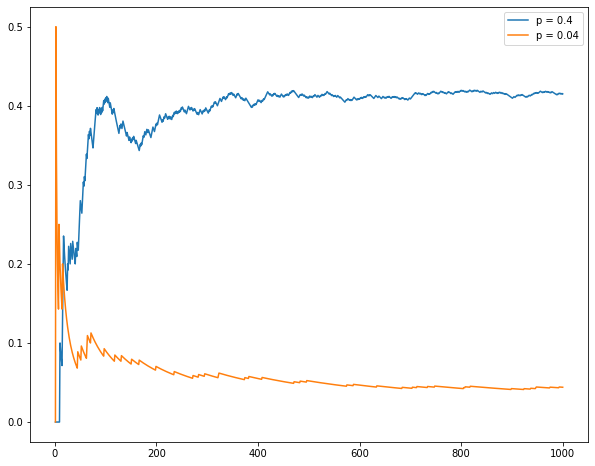
\includegraphics[width=0.5\linewidth]{images/question1/output.png}
    \caption{Proportion of heads during flipping coin for $n=1000$ times}
    \label{question1}
\end{figure}

\subsection*{Question two}

We expect that as number of experiments grow, the estimation of the $\bar{X}$ became close to the real $\mu$.
Below is the output of my code, which obeys the expectation. Here we actully have used the frequentist approach to
show the validity of our expectaion.

\begin{mdframed}
\begin{verbatim}
p = 0.4
n_expr = 1000

n = 10, X_bar = 4.17, mu = 4.0
n = 100, X_bar = 40.23, mu = 40.0
n = 1000, X_bar = 399.53, mu = 400.0
\end{verbatim}
\end{mdframed}

\subsection*{Question three}

In \autoref{question3_venn1} you can see the venn diagram for the events A and B. Both of the events A and B have
the elements 2 and 3 in common. In \autoref{question3_conv_pAB} we can see the convergance of $P(A) \times P(B)$ to $P(A \cap B)$.
It's worth mention that in this expriment $P(A)$ is converge to $\frac{3}{6}=\frac{1}{2}$, as expected; and
$P(B)$ to $\frac{4}{6}$; $P(A \cap B)$ to $\frac{2}{6}$. These values are also could be derived from theoretical calculations.

In the next part of the question, we should bring two disjoint sets and check $P(A\cap B) = P(A) \times P(B)$ for them.
we consider $A=\{6\}$ and $B=\{1,2,3,4\}$. Venn diagram corresponding these sets is in \autoref{question3_venn2}.
To show that $P(A \cap B) = P(A) P(B)$ does not hold for this case, we rerun the experiment with flipping the
coin for 1000 times. As can be seen in the figure $P(A)$ converges to $\frac{1}{6}$ and $P(B)$ to $\frac{4}{6}$.
As was expected $P(A \cap B) = 0$ and because $P(A \cap B) \neq  P(A) P(B)$ so A and B are not independant from
each other.

\begin{figure}[h]
    \centering
    \includegraphics*[width=0.4\linewidth]{images/question3/question3_venn1.png}
    \caption{Venn diagram for events A and B in Question 3}
    \label{question3_venn1}
\end{figure}

\begin{figure}[h]
    \centering
    \includegraphics*[width=0.8\linewidth]{images/question3/conv_pAb.png}
    \caption{convergance of $P(A)\times P(B)$ to $P(A\cap B)$ with increasing toss flips}
    \label{question3_conv_pAB}
\end{figure}

\begin{figure}[h]
    \centering
    \includegraphics*[width=0.4\linewidth]{images/question3/question3_venn2.png}
    \caption{Venn diagram for events A and B in Question 3}
    \label{question3_venn2}
\end{figure}

\begin{figure}[h]
    \centering
    \includegraphics*[width=0.8\linewidth]{images/question3/diverge_pAB.png}
    \caption{divergance of $P(A)\times P(B)$ to $P(A\cap B)$ with increasing toss flips, when $A \cap B = \phi$}
    \label{question3_div_pAB}
\end{figure}

\clearpage

\subsection*{Question four}

If we switch the door after monty opens one of the empty doors our chance of winning became $\frac{2}{3}$ overal.
But if we don't change our decision the change of winning becames $\frac{1}{3}$. The reseaon behind this phenomenon,
is that if we don't switch, we only had the chance to win if we had selected the true door from the beginning, but
if we switch, in $\frac{2}{3}$ of the times we win the game. Our computer simulation shows the same result.

\begin{mdframed}
\begin{verbatim}
P(success without chaning door) =  0.35
P(success with chaning door) =  0.659
\end{verbatim}
\end{mdframed}


\clearpage

\subsection*{Question five}

Using numpy and scipy packages we come up with the following results:

\begin{mdframed}
\begin{verbatim}
X~N(5,18)

P(X<9)=0.827
P(X>-3)=1-P(X<-3)=0.970
x of P(X>x)=0.05 === x of P(X<x)=0.95: 11.979
P(0<=X<4)=P(X<4)-P(X<0)=0.288
P(|X|>|x|)=0.05 => x=13.315
\end{verbatim}
\end{mdframed}

Calculation of parts a-d are clear and we omit the explanation. To calculation the value of
$P(|X|>|x|)$ we follow approach below.

\begin{eqnarray*}
    P(|X|>|x|) = P(X>x) + P(X<-x) & = & 0.05 \\
    2P(X>x) & = & 0.05 \\
    P(X<x) & = & 0.975
\end{eqnarray*}

The subsititution of $P(X<-x)$ with $P(X>x)$ is done based on symmetricity of the normal distribution. The value of
$x$ in the $P(X<x)$ is done using quantile function provided by numpy.

\clearpage

\subsection*{Question six}

\autoref{x_y} and \autoref{xy} shows the simulated values for PDF of the Questoin 3. As can be seen in the
figures for large values of bins and sample numbers the Theoretical and Simulated values are very close to each
other. Simulation and theory estimation perfectly match together in \autoref{x_y}, but in the \autoref{xy}
they are differ a bit. Increasing number of samples and number of bins could relive this situation.

\begin{figure}[h]
    \centering
    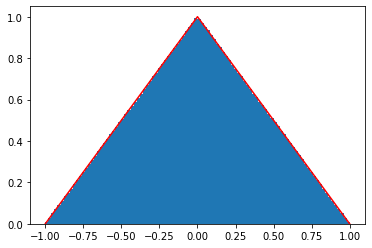
\includegraphics[width=0.5\linewidth]{images/question6/x-y.png}
    \caption{Comparison of theoretical and simulation value for $X-Y$}
    \label{x_y}
\end{figure}

\begin{figure}[h]
    \centering
    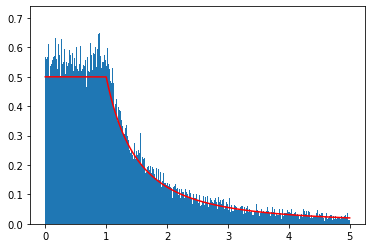
\includegraphics[width=0.5\linewidth]{images/question6/xy.png}
    \caption{Comparison of theoretical and simulation value for $X/Y$}
    \label{xy}
\end{figure}

\clearpage

\subsection*{Question seven}

Based on the text of the course book we know that:

\begin{eqnarray*}
    \Sigma = \begin{bmatrix}
        \mathbb{V}(X_1) & Cov(X_1, X_2) \\
        Cov(X_2, X_1) & \mathbb{V}(X_2)
    \end{bmatrix}
\end{eqnarray*}

So we need to calculate $\mathbb{V}(X_1)$, $\mathbb{V}(X_2)$, $Cov(X_1, X_2)=Cov(X_2, X_1)$.

\begin{eqnarray*}
    \mathbb{V}(X_1) = \mathbb{E}(X_1^2) - \mathbb{E}(X_1)^2 = 1 - 0 = 1 \\
    \mathbb{V}(X_2) = \mathbb{E}(X_2^2) - \mathbb{E}(X_2)^2 = 1 - 0 = 1 \\
    Cov(X_1, X_2) = \mathbb{E}(X_1X_2) - \mathbb{E}(X_1)\mathbb{E}(X_2) = \frac{1}{2} - 0 = \frac{1}{2}
\end{eqnarray*}

If we draw $1000$ pairs from this distribution and calculate its mean and covariance we will have
the following result, which was expected. As we increase number of samples the estimated $\mu$ and
$\Sigma$ will be closer to their real values.

\begin{mdframed}
\begin{verbatim}
mu=[0.01356353 0.01561215]

cov=[[0.97873469 0.48898598]
     [0.48898598 0.32259407]]
\end{verbatim}
\end{mdframed}

\begin{figure}[h]
    \centering
    \includegraphics*[width=0.7\linewidth]{images/question7/distribution.png}
    \caption{Samples drawn from $N(\mu, \Sigma)$ in question 7}
\end{figure}

\clearpage

\subsection*{Question eight}

Target is to find the value of $E(\sqrt{X^2+Y^2})$. We draw $n=10,000$ samples from the multivariate
normal distribution with $\mu=\begin{bmatrix}0\\0\end{bmatrix}$ and $\Sigma=\begin{bmatrix}1&0\\0&1\end{bmatrix}$.
After drawning the samples and calculations we find $E(\sqrt{X^2+Y^2})=1.259$. \autoref{dart} shows all the
landpoints of the dart and the red circle shows the mean landpoint. Most of the landpoints are close to the
coordinate which makes reasonable to have average landpoint near coordinate; but in the other hands,
some points are far away from the center. Averaging all of these values cause the mean landpoint to be a circle
with radius $1.259$.

\vspace*{1cm}

\begin{figure}[h]
    \centering
    \includegraphics*[width=0.6\linewidth]{images/question8/output.png}
    \caption{Dart average landpoint, question 8}
    \label{dart}
\end{figure}

\clearpage

\subsection*{Question nine}

Based on the text of the source book, we know that if $X_1 \sim B(n, p)$ and $X_2 \sim B(m, p)$ we conclude
$X_1 + X_2 \sim B(n+m, p)$. Also based on the text of the source book, if $X_1 \sim B(n, p_1)$ and
$X_2 \sim B(n, p_2)$ we have $X_1+X_2 \sim B(n, p_1+p_2)$. But the latter doesn't seem true.
The incorrectness of that could be shown with both theoretical approach and simulation.
Suppose we have two distributions $X_1 \sim B(n, 0.8)$ and $X_2 \sim B(n, 0.7)$. Using the statement
we can conclude $X_1+X_2 \sim B(n, 0.8+0.7=1.5)$, which is obviously wrong because the probability
of falling head in the flipping toss can't be greater than one. This was the theoretical
approval to the incorrectness of the statement. In the following parts we see in computer simulation.

\begin{itemize}
    \item $X_1 \sim B(n, p_1), X_2 \sim B(n, p_2) \centernot\implies X_1+X_2 \sim B(n, p_1+p_2)$.

    To show above statement is wrong we draw samples from their corresponding distribution and
    compare their CDF. \autoref{x1x2_bionomial} shows that CDF of these two distributions
    doesn't match and so we based on this we can't say that $X_1+X_2$ have bionomial distribution.
    We also have tried many parameters to show that $X_1+X_2$ have bionomial distribution, but
    the results was not good.

    \begin{figure}[h]
        \centering
        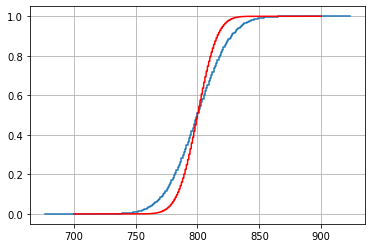
\includegraphics[width=0.6\linewidth]{images/question9/x1x2.png}
        \caption{comparison of two distributions $X_1+X_2$ (in blue) and $B(1000, 0.3+0.5=0.8)$(in red)}
        \label{x1x2_bionomial}
    \end{figure}

    \item $X_1 \sim B(n_1, p), X_2 \sim B(n_2, p) \implies X_1+X_2 \sim B(n_1+n_2, p)$.

    Following the same strategy, we can see that distribution of $X_2+X_3$ perfectly match the
    distribution of $B(n_2+n_3, p)$. (\autoref{x2x3_bionomial}) We explain the result with a simple example.
    Suppose if we have a coin and flip that $n_1$ times. The distribution stated by this phenomenon
    is bionomial with $B(n_1, p)$. What adding $X_2 \sim (n_2, p)$ means is that we flip the coin $n_2$ times more.
    It is reasonable that the resulted phenomenon have the bionomial distribution with parameters $n_1+n_2$ and $p$.

    \begin{figure}[h]
        \centering
        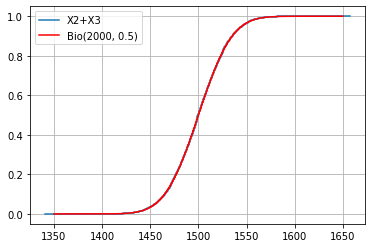
\includegraphics[width=0.6\linewidth]{images/question9/x2x3.png}
        \caption{comparison of two distributions $X_2+X_3$ (in blue) and $B(1000+2000, 0.5)$(in red)}
        \label{x2x3_bionomial}
    \end{figure}

\end{itemize}

\subsection*{Question ten}

\autoref{e_x_bar_normal} and \autoref{e_x_bar_cauchy} shows the $\bar{X}_n$ for the normal and cauchy distribution, respectively.
As can be seen there is a huge difference between the distributions. For normal distribution $\bar{X}_n$ converges to
$0$ for very large values of $n$, but this does not happen for cauchy distribution. This happens because
expectation of cauchy distribution is not defined, but expectaion of the normal distribution is defined and is equal to
$\mu$.

\begin{figure}[h]
    \centering
    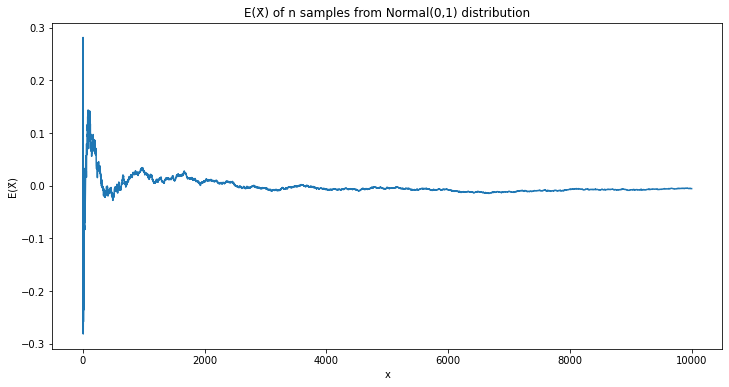
\includegraphics[width=0.8\linewidth]{images/question10/normal.png}
    \caption{$\bar{X}_n$ of $n$ samples from $\mathcal{N}(0,1)$}
    \label{e_x_bar_normal}
\end{figure}

\begin{figure}[h]
    \centering
    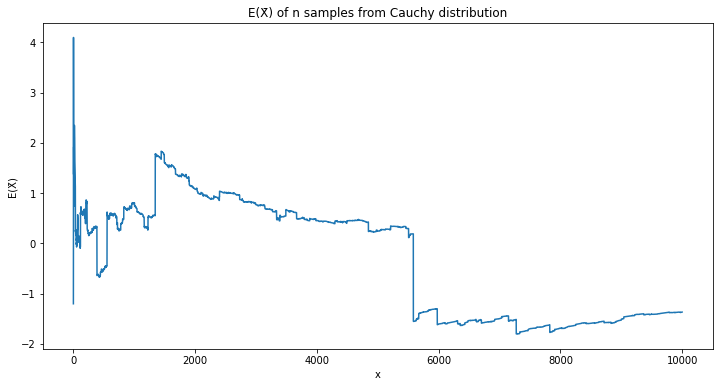
\includegraphics[width=0.8\linewidth]{images/question10/cauchy.png}
    \caption{$\bar{X}_n$ of $n$ samples from $\frac{1}{\pi(x^2+1)}$}
    \label{e_x_bar_cauchy}
\end{figure}

\clearpage

\subsection*{Question eleven}

\autoref{cdf_xi} shows the CDF for $X_i \sim \mathcal{N}(0,\frac{1}{i})$ with $i \in \{1, 100, 1000, 10000\}$.
Except $X_1$, others have very similar CDF function, which is very close to CDF of the point mass function.

\begin{figure}[h]
    \centering
    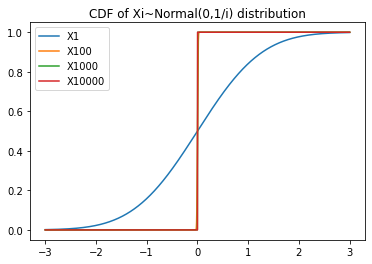
\includegraphics[width=0.5\linewidth]{images/question11/cdf.png}
    \caption{CDF for $X_i \sim \mathcal{N}(0,\frac{1}{i})$}
    \label{cdf_xi}
\end{figure}

To show that $X_i$ converges to $0$ in both probability and distribution; we show that,
$X_i$ converges to $0$ in quatratic mean. \autoref{convergance_dist_prob} shows the quadratic mean
for $X_i$. Here we have calculated $E(|X_i-0|^2)$. Because $E(X_i^2)$ converges to zero we can say
that $X_i$ converges to 0 in quantratic mean so $X_i$ converges to zero in both probability and
distribution.

\begin{figure}[h]
    \centering
    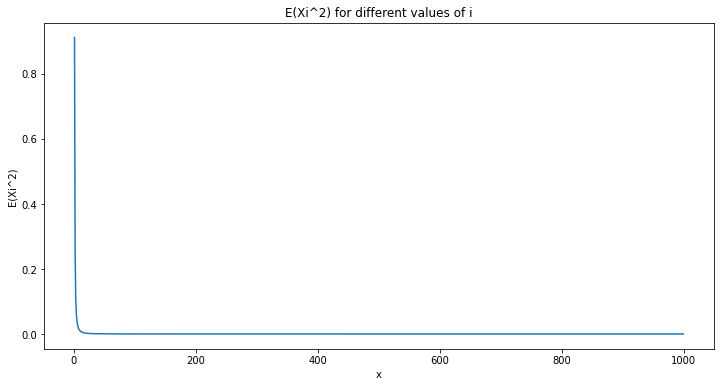
\includegraphics[width=0.5\linewidth]{images/question11/convergance_dist_prob.png}
    \caption{Convergance in quadratic mean for $X_i$ in question 11}
    \label{convergance_dist_prob}
\end{figure}

\subsection*{Question twelve}

\subsubsection*{Part a}

By drawing samples from the distribution and calcualting their mean and then
comparing the result with $p$, we see that almost always $P(|\bar{X} - p|) = 0$.
Using Chebishev's inequallity we have $P(|\bar{X} - p|) \le \frac{1}{4n\sigma^2} = 0.062$ and
Using Hoeffding's inequallity we have $P(|\bar{X} - p|) \le 2e^{-2n\sigma^2} = 0.001$. As expected
both of the upper bounds are true but the Hoeffding upper bound is tighter.

\begin{mdframed}
\begin{verbatim}
P(|X̄-p|>0.2) = 0.0
Chebishev's upperbound: 0.062
Hoeffding's upperbound: 0.001
\end{verbatim}
\end{mdframed}

\subsection*{Part b}

because of the independance of the upper bounds from $p$ both Chebishev and Hoeffding
suggest the same upper bound for the $P(|\bar{X}-p|)$. But expriments in this question also
suggests that $P(|\bar{X}-p|)$ is very close to zero. So we conclude the same statement like part a.

\begin{mdframed}
\begin{verbatim}
P(|X̄-p|>0.2) = 0.0
Chebishev's upperbound: 0.062
Hoeffding's upperbound: 0.001
\end{verbatim}
\end{mdframed}


\end{document}